%programminglanguage.tex
To be able to provide the desired functionality from the web interface, the web pages must be dynamic and able to interact with the database. There are several different programming languages to choose from. Some of the most common are ASP.NET, PHP and Java Servlets(Servlets). Due to the fact that ASP.NET is not open source \cite{aspTerms}, and the project is, this is not a feasible choice. This section will do a deeper analysis of PHP and Servlets, to argue for the best choice of programming language.

\subsection*{PHP}
PHP originally emerged in 1994 when creator Rasmus Lerdorf wrote a simple set of Common Gateway Interfaces (CGI)\footnote{The Common Gateway Interface (CGI) allows an HTTP server and a Computer-generated Imagery script to share responsibility for responding to client requests \cite{CGI}.} to track visits on his online resume, and decided to name it ``Personal Home Page Tools'' (PHP Tools). As more functionality was desired, he rewrote PHP Tools to fit his demands, and in mid 1995 he released the source code to the public.
\\In 1997 version 3.0 of PHP was released, and the name changed from ``Personal Home Page Tools'' to the recursive acronym ``PHP: Hypertext Preprocessor'' as which it is known today. This is the first version that closely resembles PHP as it exists today \cite{phpHistory}.


\subsubsection*{Key functionality}

\noindent The following list is a segment of functionality found in PHP 5.4.3. This is based on \cite{phpFunctionality}:

\begin{description}
	\item[Operating system] PHP is supported by all major operating systems, including Linux, many UNIX variants, Microsoft Windows, MAC OSX etc.
	\item[Output] PHP provides the functionality to output not only HTML, but also images, PDF files and Flash movies, all generated on the fly
	\item[Databases] PHP supports a wide range of different databases, including but no limited to MySQL, SQLite and PostgresSQL. The entire list of supported databases can be found at \url{http://www.php.net/manual/en/refs.database.php}. 
	\item[Protocols] PHP can use other service protocols than HTTP, and it is possible to open raw network sockets.
\end{description}


\subsubsection*{Requirements}

\noindent To be able to run PHP on a web server, this needs to support PHP. \href{http://www.php.net/manual/en/tutorial.requirements.php}{php.net} recommends using Apache web server, and and for database control MySQL \cite{phpReq}.

\subsection*{Java Servlets}
The first version of Servlets was created by Sun Microsystems in mid 1997, and in December 2009 version 3.0 was released\cite{servletHistory}. It was developed to use the advantages of Java to solve the problems of performance, scalability and security in CGI\cite{servletHistory2}.

\subsubsection*{Key functionality}

\noindent The following list is a segment of functionality found in Servlets. This is based on \cite{servletFunctionality}.

\begin{description}
	\item[Portability] Because servlets are written in Java, they are platform independent.
	\item[Power] Servlets can use the full functionality of core Java APIs; this includes URL access, multithreading, image manipulation, database connectivity etc.
	\item[Efficiency] When a Servlet is loaded, in remains in the servers memory as a single object instance, this makes it able to handle requests almost immediately.
	\item[Safety] Due to Servlets being written in Java, they inherit the strong type safety.
\end{description}

\subsubsection*{Requirements}

\noindent To be able to run Servlets on a web server, this needs to support Servlets. Apache has made a service to allow the execution of servlets, called \href{http://tomcat.apache.org/}{Tomcat}.


\subsection*{Comparing PHP and Servlets}
When comparing PHP and Servlets, the focus is put on efficiency and number of active sessions in both languages, as this will be the main requirements for the web interface. The following is based on \cite{servletVsPHP} - a research paper by ``IBM Tokyo Research Laboratory''.

\subsubsection*{Efficiency}
The web interface must be able to run fast and smooth, even on high load. A benchmark test is found in \autoref{fig:phpVsServlet}. The test calculates a quicksort which sorts 100 integers, A Levenshtein algorithm to measure the similarity between two strings of 56
characters and a Fibonacci execution which calculates the 15th value, with two random starting values. The setup is:

\begin{quotation}
We compared the total run time of
executing each test 10,000 times with each engine. We also executed each benchmark
an additional 10,000 times as a warm-up, before the measured test. This prevents
Java just-in-time compilation overhead from impacting the score in the Java tests.
We ran the experiment on an Intel Pentium 4 CPU at 3.40 GHz with 3GB RAM
Memory, with the Linux 2.6.17 kernel. \cite[p. 167]{servletVsPHP}
\end{quotation}

\begin{figure}[htbp]
	\centering
		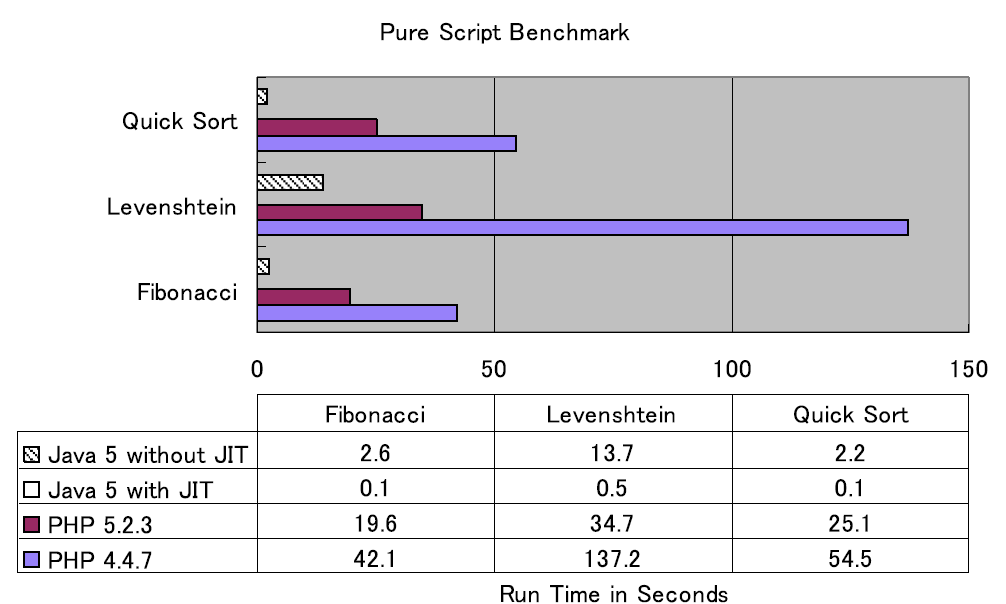
\includegraphics[width=1.00\textwidth]{images/phpVsServlet.png}
	\caption{A script benchmark calculating the average time of 10000 executions \cite{servletVsPHP}.}
	\label{fig:phpVsServlet}
\end{figure}

As seen from \autoref{fig:phpVsServlet} Servlets are faster in all tests, with and without Just In Time (JIT) compilation.

\subsubsection*{Sessions}
The web interface must be able to handle many active sessions at the same time. A test of this is shown in \autoref{fig:phpVsServlets2}\cite[p. 173]{servletVsPHP}.

\begin{quotation}
[The figure]... shows the maximum performance for each configuration and scenario, as
determined by the maximum number of simultaneous sessions (e.g., users) which can
be supported with acceptable Quality Of Service as defined by SPEC \cite[p. 173]{servletVsPHP}.
\end{quotation}

\begin{figure}[htbp]
	\centering
		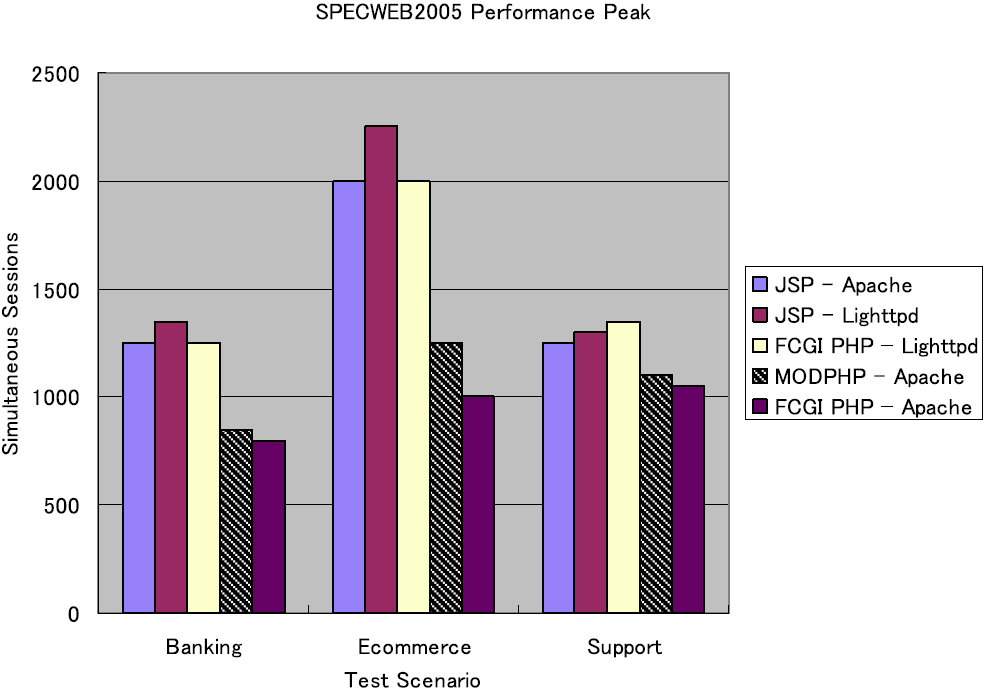
\includegraphics[width=1.00\textwidth]{images/phpVsServlets2.png}
	\caption{Simultaneous active sessions.}
	\label{fig:phpVsServlets2}
\end{figure}

\autoref{fig:phpVsServlets2} shows that 2 of 3 test cases Java Server Pages(JSP)\footnote{The elements in a Java Server Page will generally be compiled by the JSP engine into a servlet\cite{devx}.} is able to handle more active users than PHP.

The Servlets in general is more powerful than PHP, but this only comes to show when the server load is high (around 750 active sessions at the same time). Even though the efficiency of JSP is better than PHP, the following quote sums up the discussion quite well:

\begin{quotation}
When implementing a web server system which will never experience high load, or in
which performance, throughput, and reliability under high load is not an issue, then
the use of any of the analyzed languages or web servers will achieve similar
performance results. If outstanding performance and throughput is the primary goal,
then the use of JSP over PHP is advisable. However, if a 5-10\% difference in
throughput and performance is acceptable, then the implementer of a web system can
achieve similar results using either PHP or JSP. In which case, other requirements
such as developer language familiarity and programming efficiency, maintainability,
security, reliability, middleware compatibility, etc. would be the deciding factors \cite[p. 181]{servletVsPHP}.
\end{quotation}

We have chosen to implement the web interface in Servlets, due to the fact that we have a lot of experience in Java.